\zag{Эффект керра}
\thispagestyle{empty}

\subzag{Введение.}
Мы имели дело с такими средами, свойства симметрии которых
определялись внутренними свойствами вещества. Однако, действие
силовых полей может понизить симметрию среды --- превратить
изотропное тело в анизотропное.\par
В то же время, оптическое поведение вещества, находящегося в
состоянии искуственной анизотропии конечно определяется
свойствами молекул, из которых состоит вещество. Поэтому
исследование поведения вещества в силовых полях представляет
pинтерес для изучения молекул, их строения. В 1875 году Керр
установил, что прозрачное изотропное вещество становится
двоякопреломляющим под действием электрического поля (кубический
кристалл, жидкость, газ).
Двойное лучепреломление испытывают волны, распространяющиеся под
углом к направлению поля.\par
Вещество приобретает свойства одноосного кристалла. Направление
главной оптической оси совпадает с направлением поля. Это явление
отличается от {\it электрострикции}. Под {\it электрострикцией} понимается
механическая деформация тела электрическим полем: Если вещество
характеризуется скалярной величиной $\cal E$, то $(\Delta V)_{p,T}$ --
скалярное изменение удельного объёма.

%\begin{figure}[tbp]
\centerline{\hbox{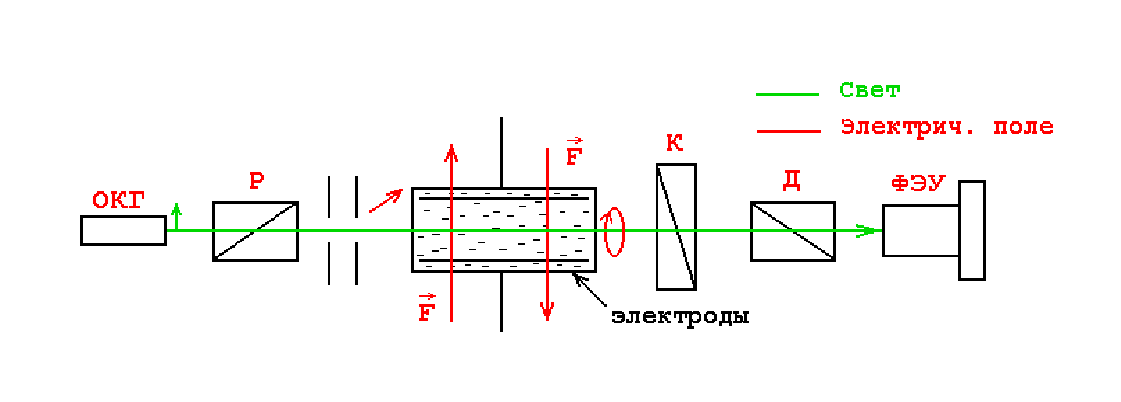
\includegraphics[scale=0.69]{Ris/ris_eps/eff_kerr/ris1.eps}}}

%\risp{6.1}{}
%\end{figure}

Эксперимент приводит к следующим закономерностям:\par\vskip 2mm
{\leftskip 1 true cm
$P$ -- направления колебаний, параллельное полю;\par
$S$ -- направление колебаний, перпендикулярное полю;\par
}
$$n_p -n_s=\gamma F^2 \eqno (6.1)$$
$$\delta=(n_p -n_s)l=\gamma l F^2 \eqno (6.2)$$\par
$\delta$ --- это разность хода на пути $l$.\par
Сдвиг фазы ${\delta \over \lambda}={\phi \over 2\pi}=BlF^2$;
$$B={\gamma \over \lambda} \eqno (6.3)$$
$B$ --- это константа для данного вещества. Вводят величину
$K$ $\left(\rm \hbox{из} (6.1) и (6.2)\right)$:
\par $$K={B\lambda \over n}={n_p - n_s \over n}{1 \over F^2}\eqno
(6.4)$$\par
Константу $K$ называют {\it константой Керра}. В зависимости от
строения и симметрии молекул $B$ и $K$ могут быть как
положительными, так и отрицательными. Порядок величины $K$ для
газов равен $10^{-15}$, для жидкостей --- $10^{-12}$ {\sl СГСЕ} единиц.
Явление Керра, как мы увидим, объясняется ориентирующим действием
поля на анизотропно поляризующиеся дипольные и бездипольные
молекулы. Теория была сначала предложена Фойгтом (электронная
теория), а затем Ланжевеном и Борном. Очевидно, что прямое
действие электрического поля на молекулу можно рассматривать
только в газе. В то время как в жидкости мы должны учитывать
ориентационное взаимодействие между молекулами.\par
\subzag{Классическая теория явления Керра для газов}
Теория Файгта основана на классической электронной теории,
сущность явления сводится к изменению собственных частей
гармонических осцилляторов в электрическом поле.\par
Для изотропной среды уравнение Лоренц-Лоренца выглядит так:
$${n^2 -1 \over n^2 +2}{M \over \rho}= $$
$$={1\over 3}{e^2 \over
m}\left\{\sum\limits_i{f_{i}^{(1)} \over \left(w_{i}^{(1)}\right)^2-w^2} +
\sum\limits_j{f_{j}^{(2)} \over \left(w_{j}^{(2)}\right)^2-w^2} +
\sum\limits_k{f_{k}^{(3)} \over \left(w_{k}^{(3)}\right)^2-w^2}\right\} \eqno
(6.5)$$
Здесь $f_{i}^{(1)},\ f_{j}^{(2)},\ f_{k}^{(3)},\ w_{i}^{(1)},\
w_{j}^{(2)},\ w_{k}^{(3)}$\ --- силы осцилляторов и частоты
колебаний электронов соответственно, характеризующие три главные
значения эллипсоида поляризуемости молекулы.\par
Файгт сводит действие поля к изменению частот колебаний
ангармонически колеблющихся электронов. Приняв уравнение движения
изотропного ангармонического осциллятора $$m\ddot x + kx-cx^3=0
\eqno (6.6)$$ Фойгт находит, что под действием поля осциллятор
становится анизотропным, и его частоты оказываются различными
по направлению поля и перпендикулярно к нему. Изменения частот
при сделанном предположении пропорциональны квадрату
напряжённости поля. Для колебаний электрона в направлении поля
смещение частоты втрое больше, чем в перпендикулярном
направлении. Отсюда Фойгт получает следующее соотношение между
$n_p$ и $n_s$:
$${n_p -n \over n_s -n}=3 \eqno (6.7)$$ однако опыт даёт для
этого отошения $${n_p -n \over n_s -n}=-2 \eqno (6.8)$$\par
Строгий квантово-механический расчёт показывает, что эффект
Фойгта существует, но его величина очень мала. Для бездипольных
молекул теория эффекта Керра была создана Ланжевеном и дополнена
затем Борном для дипольных молекул.\par
\subzag{Ориентационная теория эффекта Керра-Ланжевена-Борна}
Действие поля сводится к ориентации молекул. Такая ориентация
нарушает равномерное распределение --- при выводе постоянной среды
из молекулярных констант нельзя проводить усреднение, считая все
направления ориентации молекул равновероятными, но необходимо
приписывать  каждой ориентации определённый статистический вес,
зависящий от энергии молекулы в поле. Тепловое движение молекул
мешает молекулярной ориентации, поэтому $K=K(T)$.\par
В обычных условиях молекулы в газе подчиняются статистике
Больцмана. При наличии поля (электрического, магнитного, градиента
скорости) функция распределения по значениям потенциальной
энергии молекул в электростатическом (в частности) поле $\vec F$
равна: $$\Phi=Ce^{-{W \over KT}} \eqno (6.9)$$
где
$$W=-\sum\limits_{\sigma}p_{\sigma}^{(0)}F_{\sigma}-{1\over2}\sum\limits_{\sigma
,\tau}a_{\sigma\tau}^{(0)}F_{\sigma}F_{\tau}=-\sum\limits_{i}p_{i}^{(0)}F_{i}-{1\over2}\sum\limits_{i,j}a_{ij}^{(0)}F_{i}F_{j}
\eqno (6.10)$$
Здесь $p_{\sigma}^{(0)}$ и $p_{i}^{(0)}$, $a_{\sigma
,\tau}^{(0)}$ и $a_{i,j}^{(0)}$ --- составляющие момента и
составляющие тензора поляризуемости соответственно,
представленные в молекулярной и лабораторной системах координат.
\par Выражение (6.10) является инвариантом, а коэффициент $C$ в
(6.9) находится их условия нормировки:
$$\int\Phi d\Omega = C\int e^{-{W \over KT}}d\Omega =1 \eqno
(6.11)$$
\par Наибольшие значения напряженности поля $\vec F$, достигнутые в
эксперименте имеют порядок $10^{5}\ {\rm \hbox{вольт}\over \hbox{см}}$. Порядок
величины $p^{(0)}\sim 10^{-12}$, а порядок $a^{(0)}\sim
10^{-24}\rm \hbox{см}$. Следовательно, при обычных температурах
($T=300^{\circ}\rm \hbox{K}$), порядок ${p^{(0)}F\over KT}\sim 10^{-2}$, а
${a^{(0)}F^{2}\over KT}\sim 10^{-5}$. На этом основании при
разложении в ряд экспоненты (6.9) можно ограничиться первыми
членами в разложении
$$\Phi\simeq C\left\{ 1+{1\over
KT}\sum\limits_{\sigma}p_{\sigma}^{(0)}F_{\sigma}+{1\over
2KT}\sum\limits_{\sigma
,\tau}a_{\sigma\tau}^{(0)}F_{\sigma}F_{\tau}+{1\over
2K^2T^2}\sum\limits_{\sigma
,\tau}p_{\sigma}^{(0)}p_{\tau}^{(0)}F_{\sigma}F_{\tau}\right\}
\eqno (6.12)$$\par
Вычислим в явном виде $C$. Пусть поле $\vec F$ направлено по оси
лабораторной системы координат $z$:
$$\Phi\simeq C\left\{ 1+{F\over
KT}\sum\limits_{\sigma}p_{\sigma}^{(0)}(\sigma z)+{F^2\over
2KT}\sum\limits_{\sigma
,\tau}\left( a_{\sigma\tau}^{(0)}+{1\over
KT}p_{\sigma}^{(0)}p_{\tau}^{(0)}\right)(\sigma z)(\tau z)\right\}
\eqno (6.12\hbox{\it a})$$\par
Подставим (6.12а) в (6.11) и, принимая во внимание величины
направляющих косинусов (углы Эйлера):
$${1\over C}=\int e^{-{W\over KT}}d\Omega\simeq$$
$$\simeq \int\left\{
1+{F\over KT}\sum\limits_{\sigma}p_{\sigma}^{(0)}(\sigma z)+{F^2\over
2KT}\sum\limits_{\sigma
,\tau}\left( a_{\sigma\tau}^{(0)}+{1\over
KT}p_{\sigma}^{(0)}p_{\tau}^{(0)}\right)(\sigma z)(\tau
z)\right\}d\Omega =$$ $$=\int\limits_{0}^{2\pi}\int\limits_{0}^{2\pi}
\int\limits_{0}^{2\pi}\left\{ 1+{F\over
KT}\sum\limits_{\sigma}p_{\sigma}^{(0)}(\sigma z)+\right.$$
$$+\left.{F^2\over
2KT}\sum\limits_{\sigma
,\tau}\left( a_{\sigma\tau}^{(0)}+{1\over
KT}p_{\sigma}^{(0)}p_{\tau}^{(0)}\right)(\sigma z)(\tau
z)\right\}d\varphi d\psi \sin \vartheta d\vartheta=$$
$$=8\pi^2\left\{ 1+{F^2\over
6KT}\sum\limits_{\sigma}\left(a_{\sigma\sigma}^{(0)}+{1\over
KT}p_{\sigma}^{(0)^2}\right)\right\} \eqno (6.13)$$
и окончательно в следствие малости второго члена в (6.13):
$$C={1\over 8\pi^2}\left\{ 1-{F^2\over
6KT}\sum\limits_{\sigma}\left(a_{\sigma\sigma}^{(0)}+{1\over
KT}p_{\sigma}^{(0)^2}\right)\right\} \eqno (6.13\hbox{\it a})$$\par
С точностью до квадратичных членов:
$$\Phi={1\over 8\pi^2}\left\{ 1+{F\over
KT}\sum\limits_{\sigma}p_{\sigma}^{(0)}(\sigma z)+\right.$$
$$+\left.{F^2\over
2KT}\left[ \sum\limits_{\sigma
,\tau}\left(a_{\sigma\tau}^{(0)}+{1\over
KT}p_{\sigma}^{(0)}p_{\tau}^{(0)}\right) (\sigma z)(\tau z)-{1\over
3}\sum\limits_{\sigma}\left(a_{\sigma\sigma}^{(0)}+{1\over
KT}p_{\sigma}^{(0)^2}\right)\right]\right\} \eqno (6.12\hbox{\it b})$$\par
Мы считали до сих пор составляющие тензора поляризуемости
константами. Однако, они могут изменяться под действием поля. Мы
можем написать общее выражение оптической поляризуемости молекулы
в поле:
$$A_{\sigma\tau}=a_{\sigma\tau}+\sum\limits_{\nu}a_{\sigma\tau
,\nu}F_{\nu}+{1\over2}\sum\limits_{\nu ,\rho}a_{\sigma\tau
,\nu\rho}F_{\nu}F_{\rho}+\cdots \eqno (6.14)$$
где $a_{\sigma\tau ,\nu}=\left({\partial A_{\sigma\tau}\over
\partial F_{\nu}}\right)_{F=0}$, $a_{\sigma\tau
,\nu\rho}=\left({\partial^2
A_{\sigma\tau}\over
\partial F_{\nu}\partial F_{\rho}}\right)_{F=0}$.\par
В отсутствие поглщения света $A_{\sigma\tau}$ --- эрмитов тензор.
Следовательно, тензор III ранга $a_{\sigma\tau ,\nu}$ и тензор IV
ранга $a_{\sigma\tau ,\nu\rho}$ также должны быть эрмитовыми.\par
Вычислим средние значения составляющих тензора поляризуемости
$A_{\sigma\tau}$ в лабораторой системе координат при учете
функции распределения (6.12b). Направление $\vec F$ совпадает с
осью "$z$".
$$\overline{A_{ik}}=\sum\limits_{\sigma
,\tau}\overline{A_{\sigma\tau}(\sigma i)(\tau k)}\hskip 1 mm
\hbox{\hbox{=}\hskip -2.7 mm \raise 3 mm \hbox{$\Phi$}}
\sum\limits_{\sigma ,\tau}\int\Phi A_{\sigma\tau}(\sigma i)(\tau
k)d\Omega =$$
$$=
 \sum\limits_{\sigma ,\tau}\overline{A_{\sigma\tau}(\sigma
i)(\tau k)}+{F\over KT}\sum\limits_{\sigma\tau ,\nu}P_{\nu}^{(0)}A_{\sigma\tau}\overline{(\sigma i)(\tau k)(\nu
z)}+$$ $$+{F^2\over 2KT}\sum\limits_{\sigma\tau
,\nu\rho}\left(a_{\nu\rho}^{(0)}+{1\over KT}P_{\nu}^{(0)}P_{\rho}^{(0)}\right)
A_{\sigma\tau}\overline{(\sigma i)(\tau k)(\nu z)(\rho z)}-$$
$$-{F^2
\over 2KT}\sum\limits_{\sigma ,\tau}\left(a^{(0)}+{P^{(0)^2}\over
3KT}\right)A_{\sigma\tau}\overline{(\sigma i)(\tau k)} \eqno
(6.15)$$\par
Подставим (6.14) и с точностью до $F^2$ получим:
$$\overline{A_{ik}}=\sum\limits_{\sigma ,\tau}\overline{(\sigma
i)(\tau k)}+F\sum\limits_{\sigma\tau ,\nu}\overline{(\sigma
i)(\tau k)(\nu z)}+$$ $$+{F\over KT}\sum\limits_{\sigma\tau
,\nu}P_{\nu}^{(0)}a_{\sigma\tau}\overline{(\sigma i)(\tau k)(\nu
z)}+{F^2\over 2}\sum\limits_{\sigma\tau
,\nu\rho}a_{\sigma\tau ,\nu\rho}\overline{(\sigma i)(\tau k)(\nu z)(\rho z)}+$$
$$+{F^2\over
KT}\sum\limits_{\sigma\tau ,\nu\rho}a_{\sigma\tau
,\nu}P_{\rho}^{(0)}\overline{(\sigma i)(\tau k)(\nu z)(\rho
z)}+$$ $$+{F^2\over 2KT}\sum\limits_{\sigma\tau
,\nu\rho}\left(a_{\nu\rho}^{(0)}+{1\over
KT}P_{\nu}^{(0)}P_{\rho}^{(0)}\right)a_{\sigma\tau}\overline{(\sigma
i)(\tau k)(\nu z)(\rho z)}-$$
$$-{F^2\over 2KT}\sum\limits_{\sigma
,\tau}\left(a^{(0)}+{p^{(0)^2}\over
3KT}\right)a_{\sigma\tau}\overline{(\sigma i)(\tau k)} \eqno
(6.16)$$\par
Согласно форулам для величины произведений направляющих косинусов
различных порядков получим выражения для
$\overline{A_{xx}}=\overline{A_{yy}}$, а также для
$\overline{A_{zz}}$ и $\overline{A_{xy}}$.
$$\overline{A_{xx}}=\overline{A_{yy}}=a+F^2\left\{{1\over
30KT}\sum\limits_{\sigma}a_{\sigma\sigma}\left(a_{\sigma\sigma}^{(0)}+{1\over
KT}P_{\sigma}^{(0)^2}\right)+\right.$$
$$+\left.{1\over 15KT}\sum\limits_{\sigma
,\tau}a_{\sigma\sigma}\left(a_{\tau\tau}^{(0)}+{1\over
KT}P_{\tau}^{(0)^2}\right)-\right.$$ $$-{1\over
60KT}\sum\limits_{\sigma
,\tau}a_{\sigma\tau}\left(a_{\sigma\tau}^{(0)}+{1\over
KT}P_{\sigma}^{(0)}P_{\tau}^{(0)}\right)-$$
$$-{1\over
6KT}\sum\limits_{\sigma}\left(a^{(0)}+{P^{(0)^2}\over
3KT}\right)a_{\sigma\sigma}+{1\over
15KT}\sum\limits_{\sigma}P_{\sigma}^{(0)}a_{\sigma\sigma
,\sigma}+$$ $$\left.+{2\over 15KT}\sum\limits_{\sigma
,\tau}P_{\tau}^{(0)}a_{\sigma\sigma ,\tau}-{1\over
30KT}\sum\limits_{\sigma ,\tau}P_{\sigma}^{(0)}a_{\sigma\tau
,\tau}+\right.$$
$$+\left.{1\over 30}\sum\limits_{\sigma}a_{\sigma\sigma
,\sigma\sigma}+{1\over 15}\sum\limits_{\sigma\tau}a_{\sigma\sigma
,\tau\tau}-{1\over 60}\sum\limits_{\sigma ,\tau}a_{\sigma\tau
,\sigma\tau}\right\} \eqno (6.16\hbox{\it a})$$

$$\overline{A_{zz}}=a+F^2\left\{{1\over
10KT}\sum\limits_{\sigma}a_{\sigma\sigma}\left(a_{\sigma\sigma}^{(0)}+{1\over
KT}P_{\sigma}^{(0)^2}\right)+\right.$$
$$+\left.{1\over
30KT}\sum\limits_{\sigma
,\tau}a_{\sigma\tau}\left(a_{\sigma\tau}^{(0)}+{1\over
KT}P_{\sigma}^{(0)}P_{\tau}^{(0)}\right)\right.-$$ $$-{1\over
6KT}\sum\limits_{\sigma}a_{\sigma\sigma}\left(a^{(0)}+{P^{(0)^2}\over
3KT}\right)+{1\over
5KT}\sum\limits_{\sigma}P_{\sigma}^{(0)}a_{\sigma\sigma
,\sigma}+$$
$$+{1\over 30KT}\sum\limits_{\sigma
,\tau}a_{\sigma\sigma}\left(a_{\tau\tau}^{(0)}+{1\over
KT}P_{\tau}^{(0)^2}\right)+$$ $$\left.+{1\over 15KT}\sum\limits_{\sigma
,\tau}P_{\sigma}^{(0)}a_{\sigma\tau ,\tau}+{1\over
15KT}\sum\limits_{\sigma ,\tau}P_{\tau}^{(0)}a_{\sigma\sigma
,\tau}+\right.$$
$$+\left.{1\over 10}\sum\limits_{\sigma}a_{\sigma\sigma
,\sigma\sigma}+{1\over 30}\sum\limits_{\sigma
,\tau}a_{\sigma\sigma ,\tau\tau}+{1\over
30}\sum\limits_{\sigma ,\tau}a_{\sigma\tau ,\sigma\tau}\right\}
\eqno (6.16\hbox{\it b})$$
$$\overline{A_{xz}}=\overline{A_{zx}}=\overline{A_{yz}}=\overline{A_{zy}}=0$$
$$\hbox{(ось $z\ \parallel\ {\vec F}$)}$$
$$\overline{A_{xy}}=\overline{A_{yx}}={1\over 6}F\left(a_{\xi\eta
,\rho}-a_{\eta\xi ,\rho}+a_{\eta\rho
,\xi}-a_{\rho\eta\xi}+a_{\rho\xi ,\eta}-a_{\xi\rho
,\eta}\right)+$$ $$+{F\over
6KT}\left\{P_{\rho}^{(0)}\left(a_{\xi\eta}-a_{\eta\xi}\right)+
P_{\xi}^{(0)}\left(a_{\eta\rho}-a_{\rho\eta}\right)+
P_{\eta}^{(0)}\left(a_{\rho\xi}-a_{\xi\rho}\right)\right\} \eqno
(6.16\hbox{\it c})$$\par
Если $\overline{A_{ik}}$ вещественный, то
$\overline{A_{xy}}=\overline{A_{yx}}=0$; если комплексный, то
$\overline{A_{xy}}$ - мнимая величина. В случае электрического
поля выражения (6.16) упрощаются.\par
1). В самом деле, любая плоскость, проведенная через ось
поля $z$ является плоскостью симметрии системы. Соотношения могут
остаться неизменными при отражении от плоскости $yz$ только при
условии $A_{xy}=0$. Это условие означает одновременно
симметричность и вещественность тензоров $a_{\sigma\tau}$ и
$a_{\sigma\tau ,\nu}$.\par
В выражении (6.14) второй и третий члены связаны с линейными и
квадратичными эффектами Штарка для уровней энергии, относящимся к
внутренним колебательным и электронным движениям в молекуле. Эти
члены и характеризуют эффект Файгта. Вследствие малости эффекта
можно пренебречь тензорами $a_{\sigma\tau ,\nu}$ и
$a_{\sigma\tau ,\nu\rho}$.\par
Предположим, что в молекуляных координатах $\xi$, $\eta$, $\rho$
тензор приведен к главным осям, абщим для $a^{(0)}$ и $a$. Это
предположение строго для облости спектра, далекой от полосы
поглощения. Получаем в этом случае:
$$\overline{A_{xx}}=\overline{A_{yy}}=a+F^2\left\{{1\over
30KT}\sum\limits_{\sigma}\left(a_{\sigma}^{(0)}+{1\over
KT}P_{\sigma}^{(0)^2}\right)a_{\sigma}+\right.$$
$$+\left.{1\over
15KT}\sum\limits_{\sigma
,\tau}a_{\sigma}\left(a_{\tau}^{(0)}+{1\over
KT}P_{\tau}^{(0)^2}\right)-\right.$$ $$\left.-{1\over
6KT}\sum\limits_{\sigma}a_{\sigma}\left(a^{(0)}+{P^{(0)^2}\over
3KT}\right)\right\}=a-{F^2\over
90KT}\left\{(a_{\xi}-a_{\eta})(a_{\xi}^{(0)}-a_{\eta}^{(0)})+
\right.$$ $$+(a_{\eta}-a_{\rho})(a_{\eta}^{(0)}-a_{\rho}^{(0)})+
(a_{\rho}-a_{\xi})(a_{\rho}^{(0)}-a_{\xi}^{(0)})+{1\over
KT}\left[(a_{\xi}-a_{\eta})\left(P_{\xi}^{(0)^2}-
P_{\eta}^{(0)^2}\right)+\right.$$ $$\left.\left.+
(a_{\eta}-a_{\rho})\left(P_{\eta}^{(0)^2}-P_{\rho}^{(0)^2}\right)+
(a_{\rho}-a_{\xi})\left(P_{\rho}^{(0)^2}-P_{\xi}^{(0)^2}\right)\right]\right\}
\eqno (6.17)$$
$$\overline{A_{zz}}=a+F^2\left\{{1\over
10KT}\sum\limits_{\sigma}a_{\sigma}\left(a_{\sigma}^{(0)}+{1\over
KT}P_{\sigma}^{(0)^2}\right)+\right.$$
$$\left.+{1\over 30KT}\sum\limits_{\sigma
,\tau}a_{\sigma}\left(a_{\tau}^{(0)}+{1\over
KT}P_{\tau}^{(0)^2}\right)-\right.$$ $$\left.-{1\over
6KT}\sum\limits_{\sigma}\left(a^{(0)}+{P^{(0)^2}\over
3KT}\right)\right\}=a+{F^2\over
45KT}\left\{(a_{\xi}-a_{\eta})(a_{\xi}^{(0)}-a_{\eta}^{(0)})+
\right.$$ $$+(a_{\eta}-a_{\rho})(a_{\eta}^{(0)}-a_{\rho}^{(0)})+
(a_{\rho}-a_{\xi})(a_{\rho}^{(0)}-a_{\xi}^{(0)})+
{1\over
KT}\left[(a_{\xi}-a_{\eta})\left(P_{\xi}^{(0)^2}-P_{\eta}^{(0)^2}\right)+
\right.$$
$$\left.\left.+
(a_{\eta}-a_{\rho})\left(P_{\eta}^{(0)^2}-P_{\rho}^{(0)^2}\right)+
(a_{\rho}-a_{\xi})\left(P_{\rho}^{(0)^2}-P_{\xi}^{(0)^2}\right)\right]\right\}
\eqno (6.17\hbox{\it a})$$
$$\overline{A_{zz}}=a+2(A_1+A_2)$$
$$\overline{A_{xx}}=\overline{A_{yy}}=a-(A_1+A_2) \eqno (6.18)$$
\vskip -3 mm
$$A_1=\Theta_1{F^2\over 2}={1\over 45KT}\left\{(a_{\xi}-
a_{\eta})(a_{\xi}^{(0)}-a_{\eta}^{(0)})+
(a_{\eta}-a_{\rho})(a_{\eta}^{(0)}-a_{\rho}^{(0)})
+\right.$$
$$\left.+(a_{\rho}-a_{\xi})(a_{\rho}^{(0)}-a_{\xi}^{(0)})\right\}{F^2\over
2}$$\par
Член $A_1$ связан с анизотропией статической поляризуемости
$a^{(0)}$.
$$A_2=\Theta_2{F^2\over 2}={1\over 45K^2T^2}\left\{(a_{\xi}-
a_{\eta})\left(P_{\xi}^{(0)^2}-P_{\eta}^{(0)^2}\right)+\right.$$
$$\left.
(a_{\eta}-a_{\rho})\left(P_{\eta}^{(0)^2}-P_{\rho}^{(0)^2}\right)+
(a_{\rho}-a_{\xi})\left(P_{\rho}^{(0)^2}-P_{\xi}^{(0)^2}\right)\right\}
{F^2\over 2}$$\par
Член $A_2$ связан с постоянным дипольным моментом молекулы. Оба
члена обращаются в ноль, есль молекулы оптически изотропные.\par
Установим связь этих молекулярных констант с явлением двойного
лучепреломления, наблюдаемого экспериментально. Уравнение
Лоренц-Лоренца в отсутствие поля:
$${n_0^2-1\over n_0^2+2}={4\pi\over 3}N_1^{(0)}a \eqno
(6.19)$$\par
Когда поля наложено, число молекул $N_1$ в силу электрострикции
отлично от $N_1^{(0)}$, а показатели преломления вдоль и поперек
поля $n_p$ и $n_s$ различны.
$${n_p^2-1\over n_p^2+2}={4\pi\over 3}N_1a_p={4\pi\over
3}N_1\overline{A_{zz}} \eqno (6.19\hbox{\it a})$$
$${n_s^2-1\over n_s^2+2}={4\pi\over 3}N_1a_s={4\pi\over
3}N_1\overline{A_{xx}} \eqno (6.19\hbox{\it a})$$
$$N_1=N_1^{(0)}+\Delta N_1=N_1^{(0)}\left( 1+{1\over
4\pi}{\partial {\cal E}\over \partial p}{F^2\over 2}\right) \eqno
(6.20)$$
Дифференцируя (6.19), получим:
$${6n_0\Delta n\over (n_0^2+2)^2}={4\pi\over
3}\left(N_1^{(0)}\Delta a+{\Delta N_1\over N_1^{(0)}}\right)
\eqno (6.21)$$\par
Значения $\Delta n$ и $\Delta a$ различны для направлений,
паралельных полю и перпендикулярных полю.
Подставляя (6.18) и (6.20) получим:
$${\Delta_p n\over n_0}={n_p-n_0\over
n_0}={(n_0^2-1)(n_0^2+2)\over 6n_0^2}\left\{{1\over
8\pi}{\partial {\cal E}\over \partial p}F^2+2{A_1+A_2\over
a}\right\}$$
$${\Delta_s n\over n_0}={n_s-n_0\over
n_0}={(n_0^2-1)(n_0^2+2)\over 6n_0^2}\left\{{1\over
8\pi}{\partial {\cal E}\over \partial p}F^2-{A_1+A_2\over
a}\right\} \eqno (6.22)$$\par
Причем в выражениях для $A_1$ и $A_2$ действующее поле $F_{эфф.}$
отлично от $F$:
$$F_{эфф.}={{\cal E}+2\over 3}F \eqno (6.22\hbox{\it a})$$\par
На опыте мы наблюдаем разницу $n_p-n_s$, следовательно член,
характеризующий элетрострикцию исчезает, и это явление не играет
роли.\par
Итак, имеем для ${n_p-n_s\over n_0}$:
$${n_p-n_s\over n_0}={(n_0^2-1)(n_0^2+2)\over 2n_0^2}\cdot
{\Theta_1+\Theta_2\over a}\left({{\cal E}+2\over
3}\right)^2{F^2\over 2}\equiv {\cal K}\cdot F^2 \eqno (6.23)$$
$${\cal K}={\pi\over 27}\left({n_0^2+2\over n_0}\right)^2({\cal
E}+2)^2N_1(\Theta_1+\Theta_2)={\cal K}_1+{\cal K}_2 \eqno (6.24)$$\par
Для разреженных газов:
$${\cal K}=3\pi N_1(\Theta_1+\Theta_2)={\cal K}_1+{\cal
K}_2$$\par
Явления Керра безинерционно, практически это мгновенный эффект,
устанавливается значительно быстрее электрострикции. Можно
определить отдельно $n_p-n_0$ и $n_s-n_0$, связанные только с
явлением Керра. ${n_p-n_0\over n_s-n_0}=-2$, эти измерения
сделаны для ряда веществ и подтверждают теорию.
$$n\simeq 1+2\pi N_1a$$
$${n_p+2n_s\over 3}=n_0$$
\par $a_p+2a_s=3a\equiv b$ --- след тензора остается. Ориентация
изменяет анизотропию усредненного тензора.


\subzag{Определение компонентов тензора поляризуемости}
Определение компонентов тензора поляризуемости возможно в
молекулярной оптике благодаря соотношениям, полученным из трех
независимых экспериментов:
1) из измерения рефракции.
$$a_{\xi}+a_{\eta}+a_{\rho}=3a={3\over 2\pi N_1}(n-1)\equiv A$$
2) из измерения константы Керра.
$$2a_{\rho}-a_{\xi}-a_{\eta}={15K^2T^2{\cal K}^2\over \pi
N_1}\cdot {1\over P^{(0)^2}}\equiv B$$
3) из измерения степени деполяризации рассеянного света.
$$(a_{\xi}-a_{\eta})^2+(a_{\eta}-a_{\rho})^2+(a_{\rho}-a_{\xi})^2=
{90\Delta\over 6-7\Delta}\left({n-1\over 2\pi N_1}\right)^2\equiv
C$$\par
Величины $a_{\xi}$ и $a_{\eta}$ определяются ноднозначно.
Небходимы дополнительные соображения, вытекающие из свойств
симметрии молекулы.\par
Примером может служить бензол: $a$ в $10^{-25}\rm \hbox{см}^3$. Это
аксиально симметричная молекула:
I) $a_{\xi}=123,1$; $a_{\eta}=123,1$; $a_{\rho}=63,5$.
II) $a_{\xi}=83,3$; $a_{\eta}=83,3$; $a_{\rho}=142,9$.\par
В обоих случаях $a={1\over 3}(a_{\xi}+a_{\eta}+a_{\rho})=103,2$.
Сравним с молекулой пиримидина:

%--- input benz.tex

\centerline{\hbox{\includegraphics[scale=0.69]{Ris/ris_eps/eff_kerr/benz.eps}}}


Бензольный момент вдоль оси $\nu$, $\Delta$ --- близка к бензолу.
I) $a_{\xi}=118,8$; $a_{\nu}=108,4$; $a_{\rho}=57,3$.
II) $a_{\xi}=57,8$; $a_{\nu}=108,4$; $a_{\rho}=118,8$.\par
Для пиримидина замена CH на изоэлектронный азот N заставляет
предполакать, что $a_{\xi}$ и $a_{\nu}$ --- близки, т. е.
подходит случай I. Можем сделать вывод, что и для бензола тоже
подходит I случай.\par
Рассмотрим пример насыщенных углеводородов.
Структура парафинов представляет большой интерес:

%--- input paraf.tex
\centerline{\hbox{\includegraphics[scale=0.69]{Ris/ris_eps/eff_kerr/paraf.eps}}}

Разветвленные парафины имеют \hbox{бо \hskip -2 mm \raise 0,4 mm
\hbox{$'$}льшую} $\cal K$ и, следовательно,
\hbox{бо \hskip -2 mm \raise 0,4 mm
\hbox{$'$}льшую} аптическую анизотропию $\gamma^2$, чем нормальные
парафины. \eject \par По мене удлиннения нормальной  цепочки $\cal K$ растет
(линейно для первых 12-и членов ряда), однако, оптическая
анизотропия меняется мало, оставаясь постоянной с $n$-бутана.
Подавляющая часть молекул находится в более выгодной
энергетически транс-конфигурации (при назкой $t^{\circ}$C).
Интересны исследования $\cal K=K(\mit T^{\circ}K)$.
\par Алифатические эфиры имеют отрицательные значения $\cal K$.
Расчет по формулам дает 3 значения $a_{\xi}$, $a_{\nu}$,
$a_{\rho}$.

%--- input alif.tex
\centerline{\hbox{\includegraphics[scale=0.69]{Ris/ris_eps/eff_kerr/alif.eps}}}

 Для $\rm (CH_3)_2O$: $a_{\xi}=48,6$; $a_{\nu}=63,0$;
$a_{\rho}=43,1$.
 Для $\rm (C_2H_5)_2O$: $a_{\xi}=78,7$; $a_{\nu}=112,6$;
$a_{\rho}=70,7$.\par
Дипольный момент направлен по оси $\xi$: $P=P_{\xi}$,
перпендикулярно наибольшей пляризуемости $a_{\xi}$. $\cal K<0$.
И в парафинах и в алифатических эфирах возможно внутреннее
вращение, поэтому здесь также интересно изучать $\cal K=K(\mit
T)$: при низких температурах наиболее вероятны транс-плоские
конфигурации.\par
У тетраэдрических молекул $\rm CH_4$, $\rm CCl_4$, $\rm SnCl_4$ так
как $\gamma^2\rightarrow 0$, то и $\cal K\rightarrow 0$. Однако в
этих молекулах обращает на себя внимание сильная деформация
электронной оболочки, велика гиперполяризуемость.\par
В случае межмолекулрных водородных связей образование водородных
связей существенно влияет на константу Керра и отражается на
характере концентрационной и температурной зависимости $\cal K$.
\par I группа: Обнаружено, что у веществ, не образующих с
растворителем водородных связей зависимость $\Delta B=f(x_2)$
почти линейна, либо рост несколько увеличивается при больших
$x_2$ (начинает играть роль диполь-дипольные взаимодействия
молекул растворенного вещества и растворителя).
II группа веществ: фенол, n-нитрофенол, n-хлорфенол, --- легко
образуют водородные связи. На кривой $\Delta B=f(x_2)$
наблюдаются отколонения от теоретической зависимости. В толуоле
наблюдается автокомплексы анилина, приводящие к $B<0$, а молекулы
анилина имеют $B>0$.

%--- input anil.tex\par
\centerline{\hbox{\includegraphics[scale=0.69]{Ris/ris_eps/eff_kerr/anil.eps}}}

В растворах диоксана молекулы образуют комплекс с растворителем:

%--- input dioks.tex
\centerline{\hbox{\includegraphics[scale=0.69]{Ris/ris_eps/eff_kerr/dioks.eps}}}
\par

Для такого комплекса величина $B$ больше, чем для анилина.
Характер концентрационной зависимости можно удолветворительно
объяснить, если предположить, что молекулы анилина обладают
$B>0$, а его комплексы имеют $B<0$. В жидком анилине имеются
димеры, связанные мостиком $\rm N-H\cdots N$ (хорошее согласие
эксперимента с расчетом).\par\noindent

\subzag{Эффект Керра в жидкостях}
Электрические и оптичесткие свойства молекул весьма устойчивы,
--- дипольный момент, компонинты тензора поляризуемости остаются
такими же, как и для изолированных молекул в газе при преходе к
жидкому состоянию. В некоторых случаях, однако, деформация
электронных оболочек в конденсированной фозе --- существенна. В
жидкостях могут существовать различного рода ориентационные
взаимодействия. прерятствующие ориентации молекул в электрическом
поле. Сильным препятствием для такой ориентации может быть
диполь-дипольное взаимодействие, донорно-акцепторная связь и т.
п. Самый важный аспект нашего рассмотрения: отличие действующего
поля от внешнего. Это отличие встречается при рассмотрении:\par
$1^{\rm \hbox{ый}}$ раз --- при рассмотрении ориентации молекул
в электрическом поле. $$F_{ор.}={\cal E\mit +2\over 3}E\eqno (*)$$

$2^{\rm \hbox{ой}}$ раз --- при вычислении двойного
лчепреломления световой волны в анизотропной среде.
$$F_{Лоренца}={n^2+2\over 3}E\eqno (*)$$\par
Исследуя эти выражения Петерлин и Стюарт получили для константы
Керра
$${\cal K}={n_p-n_s\over nE^2}=3\pi
\left(\Theta_1+\Theta_2\right){N\over n^2}\left({\cal
E\mit+2\over 3}\right)^2\left({n^2+2\over 3}\right)^2\eqno (6.25)$$
\par Для жидкостей чаще пользуются константой $B={\cal K}{n\over
\lambda}$; Сравнение (6.25) с экспериментом показывает, что
теоретическое значение в $2\div 3$ разавыше экспериментального
(для нитробензола в 22 раза (!), для ацетона в 14 раз, для
ацетонитрила в 10 раз). Вернемся к газовой формуле:
$$a_p-a_s={3\over 2}(\Theta_1+\Theta_2)E^2\eqno (6.26)$$
Формула (6.25) есть результат подстановки (*) в (6.26). Однако
правильнее выбрать иной путь: Надо написать выражение энергии
молекулы в электрическом поле и подставить его в футкцию
распределения. Плотность энергии поляризованного диэлектрика:
${E{\cal D}\over 8\pi}={{\cal E}E^2\over 8\pi}$, энергия
поляризации равна разности этой энергии и энергии поля без
диэлетрика.
$$U={{\cal E}E^2\over 8\pi}-{E^2\over 8\pi}={{\cal E}-1\over
4\pi}E{E\over 2}={PE\over 2}\eqno (6.27)$$
$$P=aNF\eqno (6.28)$$ подставим в (6.27)
$$U={1\over 2}aNEF$$ энергия поляризации одной молекулы равна
$$U=-{1\over 2}aEF \eqno (6.28\hbox{\it a})$$
\par Для изотропных молекул --- это истинная энергия каждой
молекулы. Для анизотропных --- это средняя энергия
$\left(a={a_1+a_2+a_3\over 3}\right)$. Найдем выражение для
мгновенной энергии молекулы в электрическом поле. Для газов мы
имели (неполярные молекулы ориентируются электрическом поле
по направлению поля).
$$U=-{1\over 2}\left(a_1E_1^2+a_2E_2^2+a_3E_3^2\right)=-{E^2\over
2}\left[a_1(1E)^2+a_2(2E)^2+a_3(3E)^2\right]$$
где $E_1$, $E_2$, $E_3$ --- проекции вектора $\vec E$ на главные
оси эллипсоида поляризуемости. Заменим $E^2$ на $EF$:
$$U_1=-{1\over
2}\left[a_1\cos^2(1E)+a_2\cos^2(2E)+a_3\cos^2(3E)\right]E\cdot
F\eqno (6.29)$$
\par Для полярных молекул полная поляризуемость состоит из $a$ и
$a_{ор.}={\mu^2\over 3KT}$. Для средней энергии диполя в жидкости
по аналогии с (6.28) напишем:
$$U=-{1\over 2}{\mu^2\over 3KT}E\cdot F \eqno (6.30)$$
Отсюда следует, что мгновенная энергия диполя должна зависеть от
действующего поля\footnote{*}{Если умножить (6.31) на
$e^{\left(-{U\over KT}\right)}$ и проинтегрировать по всем углам
(6.30)}:
$$U_2=-\mu\sqrt{EF}\cos\Theta \eqno (6.31)$$
Теперь, если при выводе выражения $a_p-a_s$ мы подставим вместо
полной энергии сумму $U_1+U_2$, то получим:
$$a_p-a_s={3\over 2}(\Theta_1+\Theta_2)E\cdot F={2\over
3}(\Theta_1+\Theta_2)\left({\cal E\mit +2\over 3}\right)E^2\eqno
(6.32)$$
Как видим множитель ${\cal E\mit +2\over 3}$ стоит в первой
степени. Эта формула с более строгим выводом было впервые
получена В.А. Замковым.
Здесь приведены рассуждения М.Ф. Вукса. Жидкость, помещенная в
электрическое поле становится анизотропной. Петерлин и Стюарт
записали уравнения Лоренц-Лоренца для анизотропной среды:
$${n_p^2-1\over n_p^2+2}={4\pi\over 3}N_1a_p;\hskip 3 mm
{n_s^2-1\over n_s^2+2}={4\pi\over 3}N_1a_s$$
и получили
$$n_p-n_s={2\pi N_1\over n}(a_p-a_s)\left({n^2+2\over 3}\right)
\eqno (6.33)$$
\par В анизотропной среде действующее поле $F_i={n^2+2\over 3}E$
--- изотропно. М.Ф. Вукс показал, что уравнение Лоренц-Лоренца
для жидкости в этом случае имеет тот же вид, что и для одноосного
кристалла:
$${n_p^2-1\over n^2+2}={4\pi\over 3}N_1a_p;\hskip 3 mm
{n_s^2-1\over n^2+2}={4\pi\over 3}N_1a_s \eqno (6.34)$$
Вычитая из первого равенства второе, получим
$${n_p^2-n_s^2\over n^2+2}={(n_p+n_s)(n_p-n_s)\over
n^2+2}={2n(n_p-n_s)\over n^2+2}={4\pi\over 3}N_1(a_p-a_s)$$
$$n_p-n_s={2\pi N_1\over n}(a_p-a_s){n^2+2\over 3}\eqno (6.35)$$
Обратите внимание, что множитель ${n^2+2\over 3}$ стоит в первой
степени. Соединяя (6.32) и (6.35) получаем:
$${\cal K}={n_p-n_s\over nE^2}=3\pi(\Theta_1+\Theta_2){N_1\over
n^2}\left({{\cal E}+2\over 3}\right)\left({n^2+2\over
3}\right)\eqno (6.36)$$
\par В отличие от Петерлина и Стюарта у множителей
${{\cal E}+2\over 3}$ и ${n^2+2\over 3}$ первые степени.
$$B={n_p-n_s\over \lambda E^2}=3\pi(\Theta_1+\Theta_2){N_1\over
n\lambda}\left({{\cal E}+2\over 3}\right)\left({n^2+2\over
3}\right) \eqno (6.37)$$
\par Эту формулу надо подвергнуть дальнейшим преобразованиям,
учитывая, что электронная поляризация всегда происходит в поле
Лорентца $F_Л={n_{\infty}^2+2\over 3}E$, поэтому $\left({{\cal
E}+2\over 3}\right)$ в формуле (6.37) надо отнести только ко
второму слагаемому (дипольному), а в первом множитель $\left({{\cal
E}+2\over 3}\right)$ заменить на $\left({n_{\infty}^2+2\over
3}\right)$, но так как $n_{\infty}$ нам неизвестен, мы заменяем
его на ${\cal E}_{\infty}$, высокочстотный предел ${\cal E}$.
$${n_{\infty}^2-1\over n_{\infty}^2+2}={4\pi\over 3}a\eqno
(6.38)$$ $$ {a_1^0\over a_1}={a_2^0\over a_2}={a_3^0\over
a_3}={n_{\infty}^2-1\over n^2-1}\cdot {n^2+2\over
n_{\infty}^2+2}\equiv A \eqno (6.39)$$
$$\Theta_1={1\over
45KT}A\left[(a_1-a_2)^2+(a_1-a_3)^2+(a_2-a_3)^2\right]={2A\over
45KT}\gamma^2\eqno (6.40)$$
Для неполярных жидкостей $n_{\infty}^2 \sim {\cal E}$ и $A \simeq
1$. Для полярных жидкостей ${\cal E}<10 \rightarrow A=1$;\par
\noindent $20>{\cal E}>10 \rightarrow A=1,05\div 1,10$.\par
Для неполярных жидкостей:
$$B={2\pi\over 15KT}\gamma^2{N_1\over n\lambda}\left({{\cal
E}+2\over 3}\right)\left({n^2+2\over 3}\right)\eqno (6.41)$$
\par Для полянрых жидкостей:
$$B=\left\{{2\pi\over 15KT}A\gamma^2\left({{\cal
E}_{\infty}+2\over 3}\right)\left({n^2+2\over 3}\right)+\right.$$
$$\left.+{\pi\over
15K^2T^2}\left[(a_1-a_2)(p_1^2-p_2^2)+(a_1-a_3)(p_1^2-p_3^2)+\right.\right.$$
$$+\left.\left.(a_2-a_3)(p_2^2-p_3^2)\right]
\cdot \left({{\cal E}+2\over 3}\right)\left({n^2+2\over
3}\right)\right\}{N_1\over n\lambda}\eqno (6.42)$$


\subzag{Экспериментальное изучение компонентов
эллипсоида поляризуемости в газах по эффекту Керра}

\markright{\hfill Экспериментальное изучение компонентов эллипсоида поляризуемости \hfill}

Из сравнения экспериментальных результатов с формулами (6.41) и
(6.42) порядок измеряемой величины ${\cal K}$ находится в хорошем
согласии с теорией. Подтверждается температурная зависимость как
для дипольных, так и для недипольных газов. Подтверждается
зависимость от напряженности поля и от длины волны света. В
большинстве случаев ${\cal K}>0$, но для $\rm SO_2,\ (CH_3)_2O,\
(C_2H_5)_2O,\ CHCl_3$ оказывается, что ${\cal K}<0$. Для
объяснения этого факта рассмотрим выражения для ${\cal K_1}$ и ${\cal
K}_2$:
$${\cal K}_1= 3\pi N_1\Theta_1={\pi N_1\over
15KT}\left\{(a_{\xi}-a_{\eta})(a_{\xi}^{0}-a_{\eta}^{0})+\right.$$
$$+\left.(a_{\eta}-a_{\rho})
(a_{\eta}^0-a_{\rho}^0)+(a_{\rho}-a_{\xi})(a_{\rho}^0-a_{\xi}^0)\right\}$$
$${\cal K}_2= 3\pi N_1\Theta_2={\pi N_1\over
45KT}\left\{(a_{\xi}-a_{\eta})(P_{\xi}^{0^2}-P_{\eta}^{0^2})+\right.$$
$$+\left.(a_{\eta}-a_{\rho})
(P_{\eta}^{0^2}-P_{\rho}^{0^2})+(a_{\rho}-a_{\xi})(P_{\rho}^{0^2}-P_{\xi}^{0^2})\right\}$$
\par В области, далекой от собственного поглощения,
последовательность значений $a_{\xi},\ a_{\eta},\ a_{\rho}$ и
$a_{\xi}^0,\ a_{\eta}^0,\ a{\rho}^0$ по величине одинакова ${\cal
K}>0$. Отрицательной может быть только величина ${\cal K}_2$, а
${\cal K}_1>{\cal K}_2$ всегда. ${\cal K}_2$ будет меньше нуля в
случае несовпадения по величине последовательностей $P_{\xi},\
P_{\eta}, P_{\rho}$ и $a_{\xi},\ a_{\eta},\ a_{\rho}$.\par
Можно упростить выражение для ${\cal K}_2$ в области, далекой от
собственного поглощения:
$${a_{\xi}^0\over a_{\xi}}={a_{\eta}^0\over
a_{\eta}}{a_{\rho}^0\over a_{\rho}}={n_{\infty}^2-1\over
n^2-1}\simeq {n_{\infty}-1\over n-1}$$
Для недипольных веществ:
$${\cal K}_1={\pi N_1\over 15KT}\cdot {n_{\infty}-1\over
n-1}\left\{(a_{\xi}-a_{\eta})^2+(a_{\eta}-a_{\rho})^2+(a_{\rho}-a_{\xi})^2
\right\}$$
$${\cal K}_1={2\pi N_1\over 15KT}\cdot{n_{\infty}-1\over
n-1}\gamma^2$$
Анизотропия $\gamma^2$ может быть выражена через степень
деполяризации рассеянного света и рефракцию:
$$\gamma^2=5\alpha^2{\Delta\over 6-7\Delta}={45\over
4\pi^2N_1^2}(n-1)^2{\Delta\over 6-7\Delta}$$
$${\cal K}_1={3\over 2KT}{(n_{\infty}-1)(n-1)\over \pi N_1}\cdot
{\Delta\over 6-7\Delta}$$
\par Для недипольных молекул ${\cal K}_1={\cal K}$, т. е. ${\cal
K}$ может быть определена из степени деполяризации рассеянного
света.\par
Для молекул со значительным дипольным моментом ${\cal K}_1>{\cal
K}_2$ и ${\cal K}$ может быть непосредственно вычисена из
$\Delta$, $n$ и $P^{(0)}$ только в случае аксиальной симметрии
эллипсоида поляризуемости, когда $a_{\xi}=a_{\eta}\not =a_{\rho}$.
$${\cal K}_1={2\pi\over 15KT}{n_{\infty}-1\over
n-1}(a_{\xi}-a_{\rho})^2$$
$${\cal K}_2={\pi N_1\over
15KT}(a_{\xi}-a_{\rho})^2\left\{P_{\xi}^{(0)^2}+P_{\eta}^{(0)^2}+P_{\rho}^{(0)^2}\right\}$$
В молекулах с аксиальной симметрией дипольный момент направлен
вдоль выделенной оси симметрии $\rho$, следовательно
$P_{\xi}=P_{\eta}=0$ и окончательно
$${\cal K}_2={2\pi\over
15KT}(a_{\rho}-a_{\xi})^2P_{\rho}^{(0)^2}={n-1\over
10K^2T^2}\sqrt{{5\Delta\over 6-7\Delta}}P^{(0)^2}$$
\par Знак ${\cal K}_2$ зависит от знака
$\gamma=a_{\rho}-a_{\xi}$. Приведем примеры для молекул с
аксиальной симметрией $\rm HCl,\ CH_3Cl,\ CHCl_3$. В первых двух
случаях направление дипольного момента мовпадает с осью
наибольшей поляризуемости; в $\rm CHCl_3$ дипольный момент,
совпадающий с осью симметрии, перпендикулярен к оси наибольшей
поляризуемости.\par
Если молекула плоская, и дипольный момент лежит в плоскости $\xi,\
\rho$ и образует угол $\varphi$ с осью $\rho$, то:
$P_{\xi}^{(0)}=P^{(0)}\sin\varphi$; $P_{\eta}^{(0)}=0$;
$P_{\rho}^{(0)}=P^{(0)}\cos\varphi$.
$${\cal K}_1={\pi N_1\over 15KT}P^{(0)^2}\left[3\cos^2\varphi
(a_{\rho}-a_{\xi})+2a_{\xi}-a_{\eta}-a_{\rho}\right] \eqno (**)$$
и если $\varphi =0$, то
$${\cal K}_2={\pi N_1\over
15K^2T^2}P^{(0)^2}(2a_{\rho}-a_{\eta}-a_{\xi}) \eqno (*)$$
\par Для дипольных молекул с аксиальной симметрией:
$$(a_{\rho}-a_{\xi})^2={15KT\over 2\pi N_1}\cdot {n-1\over
n_{\infty}-1}{\cal K}$$
$$a_{\rho}+2a_{\xi}={3\over 2\pi N_1}(n-1)$$
\par Стоит заметить, что знак $a_{\rho}-a_{\xi}$ неопределен.
Если аксиально симметричная молекула обладает дипольным моментом,
то для определения $a_{\rho}$ и $a_{\xi}=a_{\eta}$ из постоянной
Керра надо знать постоянный дипольный момент $\vec P^{(0)}$. Если
известно расположение вектора $\vec P^{(0)}$ по отношению к
главным осям поляризуемости $(**, *)$, то можно сопоставляя
значения ${\cal K},\ \Delta , n$ и $P^{(0)}$ можно определить все
три значения $a_{\xi},\ a_{\eta},\ a_{\rho}$.\par
Если ${\cal K}_2$ выражается $(*)$, то имеем для рефракции:
$$a_{\xi}+a_{\eta}+a_{\rho}=3a={3\over 2\pi N_1}(n-1)$$
\par Для эффекта Керра:
$$2a_{\rho}-a_{xi}-a_{\eta}={15K^2T^2{\cal K}_2\over \pi N_1}\cdot
{1\over P^{(0)^2}}$$
\par Для изменения степени деполяризации света:
$$(a_{\xi}-a_{\eta})^2+(a_{\eta}-a_{\rho})^2+(a_{\rho}-a_{\xi})^2={90\Delta\over
6-7\Delta}\left({n-1\over 2\pi N_1}\right)^2$$
\par Таким образом Стюарт определил компоненты эллипсоида
поляризуемости многих молекул\footnote{$^1$}{см. {\it Стюарт}
<<Строение молекул>>.}

\subzag{Релаксация эффекта Керра}
Мы видели, что релаксация диэлектрической поляризации в
переменном поле зависит от молекулярных свойств жидкого
диэлектрика. В теории Дебая показано, что процесс дизориентации
молекулярных диполей происходит из-за вращательной диффузии.
Время релаксации дипольной поляризации $\tau_{\cal D}={1\over
2{\cal D}}$; ${\cal D}$ --- коэффициент вращательной
диффузии.
Явление Керра устанавливается через некоторое время после
включения поля, после его выключения для двойного лучепреломления
характрено некоторое время спада, время релаксации эффекта Керра
--- $\tau_{\cal K}$. Под действием электрического поля молекулы
ориентируются (с одновременным дезориентирующим действием
теплового движения). Механизм дезориентации - {\it вращательная
диффузия}. Напишем уравнение поступательной диффузии:
$$J=-{\cal D}\hbox{grad} N+{\cal V}N \eqno (6.43) $$
где ${\cal D}$ --- коэффициент поступательной
диффузии;\par\noindent $N$ ---
число частиц в единице объема с координатой $x$,\par\noindent ${\cal V}$
--- средняя скорость движения под действием силы. ${\cal
V}=qF=-q\hbox{grad}U$; $q$ --- подвижность молекулы, $U$ ---
потенциальная энергия молекулы во внешнем поле.
$$J=-{\cal D}\hbox{grad}N-qN\hbox{grad}U \eqno (6.44)$$\par
Уравнение сохранения числа частиц:
$${\partial J\over \partial x}+{\partial N\over \partial t}=0$$
продифференцировав (6.44) и заменяя ${\partial J\over \partial x}$
на $-{\partial N\over \partial t}$ получим:
$${\partial N\over \partial t}=\hbox{div}({\cal
D}\hbox{grad}N+qN\hbox{grad}U) \eqno (6.45)$$
Это уравнение поступательной диффузии.\par
Ограничимся рассмотрением молекул с аксиальной симметрией:
$a_1\equiv a_{\parallel}$ вдоль оси
симметрии;
$a_{2}=a_3\equiv a_{\perp}$; дипольный момент направлен по оси
симметрии.\par
Ориентационная энергия в поле:
$$U=U_1+U_2=-{E^2\over 2}(a_{\parallel}-a_{\perp})\cos^2\Theta
-pE\cos\Theta$$
$\Theta$ --- угол между $\vec p$ и $\vec E$. Перейдем от (6.45) к
уравнению вращательной диффузии, произведя замену $N\rightarrow
\Phi N$ (где $\Phi$ --- функция распределения молекул по углам
ориентации).
$${\partial\Phi\over \partial t}=\hbox{div}({\cal
D}_r\hbox{grad}\Phi-q\Phi\hbox{grad}U) \eqno (6.46)$$
${\cal D}_r$ --- коэффициент вращательной диффузии.
\par В 1905 Эйнштейном было получен соотношение:
$${\cal D}_r=qKT$$
\par Если на частицы кроме градиента концентрации действует
внешняя сила $F$, то $q$ --- подвижность частиц, т. е. $V=qF$.
Величина, обратная $q$ называется коэффициентом трения
$\xi={1\over q}$; Для обратных частиц, при поступательном
движении $\xi=6\pi r_0 \eta$, где $\eta$ - вязкость.\par
Для вращательного движения, если $\xi_r$ --- коэффициент
вращательного трения:
$$\xi_r=8\pi r_0^3\eta$$
\par Формула Эйнштейна-Дебая-Стокса:
$$\tau_{\cal D}={4\pi n_0^3\eta\over KT}\hskip 0.7 cm V\not
=r_0^3$$
Имеется ввиду Ван-дер-Ваальсовский радиус молекулы, граничные
условия {\it slip} или {\it stick}, это приводит к эффективному объему
$V$*.\par
Преобразуем выражение (6.46):
$${d\Phi\over dt}={\cal D}_r\hbox{div}\,\hbox{grad}\Phi+{{\cal
D}_r\over KT}\Phi\hbox{div}\,\hbox{grad}U+{{\cal D}_r\over
KT}\hbox{grad}\Phi\,\hbox{grad}U \eqno (6.47)$$
В сферических координатах $\Phi=Phi(\Theta)$ и $U=U(\Theta)$:
$$\hbox{div}\,\hbox{grad}\Phi\equiv
{1\over\sin\Theta}\cdot{\partial\over\partial\Theta}\left(\sin\Theta{\partial
\Phi\over\partial\Theta}\right)$$
$${1\over {\cal D}_r}\cdot {\partial\Phi\over\partial
t}={1\over\sin\Theta}\cdot
{\partial\over\partial\Theta}\left(\sin\Theta
{\partial\Phi\over\partial\Theta}\right)+{\Phi\over KT}\cdot
{1\over\sin\Theta}\cdot
{\partial\over\partial\Theta}\left(\sin\Theta{\partial
U\over\partial\Theta}\right)+{1\over KT}\cdot
{\partial\Phi\over\partial\Theta}{\partial U\over\partial\Theta}
\eqno (6.48)$$
\par Для неполярных жидкостей:
$$U=-{E^2\over 2}(a_{\parallel}-a_{\perp})\cos^2\Theta \eqno
(6.49)$$
$$\Phi=Ae^{-{U\over KT}} \eqno (6.50)$$
Так как $U<<KT$, разложим $\Phi$ в ряд:
$$\Phi\simeq A\left[1+{E^2\over
2KT}(a_{\parallel}-a_{\perp})\cos^2\Theta\right] \eqno (6.51)$$
$$\int\Phi d\Omega=A\int e^{-{U\over KT}}d\Omega=1 \eqno (6.52)$$
$${1\over A}=\int e^{-{U\over
KT}}d\Omega=\int\limits_{0}^{\pi}\left[1+{E^2\over
2KT}(a_{\parallel}-a_{\perp})\cos^2\Theta\right]2\pi\sin\Theta
d\Theta$$
$${1\over A}=4\pi\left[1+{E^2\over
2KT}(a_{\parallel}-a_{\perp}){1\over3}\right]$$
$$A={1\over4\pi}\cdot {1\over 1+{E^2\over
2KT}(a_{\parallel}-a_{\perp}){1\over3}}={1\over
4\pi}\left[1-{E^2\over
2KT}(a_{\parallel}-a_{\perp}){1\over3}\right] \eqno (6.53)$$
$$\Phi={1\over 4\pi}\left[1+{E^2\over
2KT}(a_{\parallel}-a_{\perp})\left(\cos^2\Theta-{1\over3}\right)\right]
\eqno (6.54)$$\par
Такой вид имеет $\Phi$ в постоянном поле до момента его
выключения ($t=0$). После выключения поля $\Phi$ начнет
убывать:
$$\Phi={1\over 4\pi}\left[1+\Psi (t){E^2\over
2KT}(a_{\parallel}-a_{\perp})\left(\cos^2\Theta-{1\over3}\right)\right]
$$ где $\Psi(t)=e^{-{t\over\tau_k}}$ - закон убывания;
$$\Phi={1\over 4\pi}\left[1+e^{-{t\over\tau_k}}{E^2\over
2KT}(a_{\parallel}-a_{\perp})\left(\cos^2\Theta-{1\over3}\right)\right]
\eqno (6.55)$$
Подставим функцию распределения $\Phi$ в уравнение диффузии
(6.48). В данный момент $t=0$ поле выключено, U=0:
$${1\over{\cal
D}_r}{\partial\Phi\over\sin\Theta}={1\over\sin\Theta}
{\partial\over\partial\Theta}\left[\sin\Theta{\partial\Phi\over\partial\Theta}
\right]={\cos\Theta\over\sin\Theta}{\partial\Phi\over\partial\Theta}+{\partial^2\Phi\over\partial\Theta^2}
\eqno (6.56)$$
$${\partial\Phi\over\partial
t}=-{1\over\tau_k}e^{-{t\over\tau_k}}{E^2\over2KT}(a_{\parallel}-a_{\perp})\left(\cos^2\Theta-{1\over3}\right)$$
$${\partial\Phi\over\partial
\Theta}=-e^{-{t\over\tau_k}}{E^2\over2KT}(a_{\parallel}-a_{\perp})2\sin\Theta\cos\Theta$$
$${\partial^2\Phi\over\partial
\Theta^2}=-e^{-{t\over\tau_k}}{E^2\over2KT}(a_{\parallel}-a_{\perp})2\cos2\Theta$$
\par подставим в (6.56):
$${1\over {\cal
D}_r\tau_k}\left(\cos^2\Theta-{1\over3}\right)=2\cos^2\Theta+2\cos2\Theta$$
$${1\over {\cal
D}_r\tau_k}\left(\cos^2\Theta-{1\over3}\right)=6\left(\cos^2\Theta-{1\over3}\right)
\hskip 3 mm \Longrightarrow\hskip 3 mm {1\over {\cal
D}_r\tau_k}=6$$
$$\tau_k={1\over6{\cal D}_r} \eqno (6.57)$$
\par так как $\tau_{\cal D}={1\over 2{\cal D}_r}$, то
$$\tau_{k}={1\over3}\tau_{\cal D} \eqno (6.58)$$\par
Это можно перенести и на случай полярных жидкостей, но в этом
случае, кроме релаксации эффекта Керра будет наблюдаться и
релаксация дипольной поляризации. Для времени релаксации эффекта
Керра не имеет значения, обладает ли молекула дипольным моментом.
Наличие значительной проводимости в жидкости при сильных
постоянных полях ($10^5\rm\ {\hbox{вольт}\over \hbox{см}}$) затрудняет изучение
эффекта Керра. Сильные поля вызывают нагревание жидкости, ---
появляются сильные конвекционные потоки и неоднородности,
искажающие световое поле (пространственный заряд, двойной
электрический слой на границе жидкость-металл). Альтернативой
могут служить импульсные методы, слабые переменные поля.

\subzag{Явление Керра в переменном поле (неполярные жидкости)}
В переменном поле $E=E_0\cos wt$ задача сводится к решению
уравнения (6.48):
$${1\over {\cal D}}\cdot {\partial\Phi\over\partial
t}={1\over\sin\Theta}{\partial\over\partial\Theta}\left(\sin\Theta{\partial\Phi\over\partial\Theta}\right)+
{\Phi\over
KT}{1\over\sin\Theta}{\partial\over\partial\Theta}\left(\sin\Theta{\partial
U\over\partial\Theta}\right)+{1\over KT}\cdot
{\partial\Phi\over\partial\Theta}{\partial U\over\partial\Theta}$$
\par Как мы видели для энергии молекулы в электрическом поле
справедливо выражение (6.49):
$$U=-{E^2\over2}(a_{\parallel}-a_{\perp})\cos^2\Theta$$
$$E^2=E_0^2\cos^2wt=E_0^2{1+\cos2wt\over2}$$
$$U=-{E_0^2\over2}(a_{\parallel}-a_{\perp})\cos^2\Theta{1+cos2wt\over2}$$
\par Перепишем уравнение диффузии (6.48) в развернутом виде:
$${1\over {\cal D}}\cdot {\partial\Phi\over\partial
t}={\cos\Theta\over\sin\Theta}{\partial\Phi\over\partial
t}+{\partial^2\Phi\over\partial\Theta^2}+{\Phi\over
KT}\left({\cos\Theta\over\sin\Theta}{\partial
U\over\partial\Theta}+{\partial^2
U\over\partial\Theta^2}\right)+{1\over KT}{\partial
U\over\partial\Theta}\cdot {\partial\Phi\over\partial\Theta}=$$
$$={\cos\Theta\over\sin\Theta}\cdot
{\partial\Phi\over\partial\Theta}+{\partial^2\Phi\over\partial\Theta^2}+{E_0^2\over
KT}(a_{\parallel}-a_{\perp}){1+cos2wt\over2}\times$$
$$\times\left\{(\cos^2\Theta+\cos2\Theta)
\Phi+{\sin2\Theta\over2}\cdot
{\partial\Phi\over\partial\Theta}\right\}$$
\par заменяя $\cos2\Theta$ на $(2\cos^2\Theta-1)$ получим:
$${1\over {\cal D}}\cdot {\partial\Phi\over\partial t}=
{\cos\Theta\over\sin\Theta}{\partial\Phi\over\partial\Theta}+
{\partial^2\Phi\over\partial\Theta^2}+{E_0^2\over
KT}(a_{\parallel}-a_{\perp}){1+\cos2wt\over2}\times$$
$$\times\left\{(3\cos^2\Theta
-1)+{\sin2\Theta\over2}{\partial\Phi\over\partial\Theta}\right\}
\eqno (6.59)$$
\par Решение этого уравнения сводится к нахождению функции
$\Phi$. В случае постоянного поля
$$\Phi={1\over
4\pi}left[1+{E^2\over2KT}(a_{\parallel}-a_{\perp})\left(\cos^2\Theta-{1\over3}\right)
\eqno (6.54)$$
\par При переменном поле функция $\Phi$ будет отставать по фазе
от мгновенного значения поля, что приледет и к изменению
амплитуды. Подставим в (6.54) вместо $E^2=E_0^2{1+\cos2wt\over2}$
выражение
$E^2=E_0^2{A+B\cos(2wt-\delta)\over2}$:
$$\Phi={1\over4\pi}\left\{1+{E_0^2\over2KT}{A+B\cos(2wt-\delta)\over2}(a_{\parallel}-a_{\perp})
\left(\cos^2\Theta-{1\over3}\right)\right\} \eqno (6.60)$$
\par Для определения $A,\ B$ и $\delta$ подставим $\Phi$ и ее
производные по $t$ и $\Theta$ в формулу (6.59). Сравнивая члены с
одинаковой зависимостью от времени и учитывая условие
${a_{\parallel}-a_{\perp}\over2KT}E_0^2<<KT$, находим:
$$A=1;\hskip 3 mm B={1\over\sqrt{1+w^2\tau_k^2}};\hskip 3 mm
\hbox{tg}\delta=w\tau_k,\ \left(\tau_k={1\over6{\cal D}}\right) \eqno (6.61)$$
\par Окончательно для функции $\Phi$ имеем:
$$\Phi={1\over4\pi}\left\{1+\left[1+{\cos(2wt-\delta)\over\sqrt{1+
w^2\tau_k^2}}\right]{E_0^2\over4KT}(a_{\parallel}-a_{\perp})\left(\cos^2\Theta
-{1\over3}\right)\right\}\eqno (6.62)$$
\par С помощью $6.62$ можно рассчитать постоянную Керра.
Она оказывается пропорциональной переменной части этой функции:
$${\cal K}^*={\cal
K}\left\{1+{\cos(2wt-\delta)\over\sqrt{1+w^2\tau_k^2}}\right\}\eqno
(6.63)$$
${\cal K}^*$ --- мговенное значение постоянной Керра. Это
функциональная зависимость. Мгновенное значение меняется с
удвоенной частотой $2w$. Величина $\cos(2wt-\delta)$ изменяется
при заданной частоте $w$ от (+1) до (-1) и мгновенное значение
постоянной Керра в пределах
$${\cal K}_+^*={\cal
K}\left\{1+{1\over\sqrt{1+w^2\tau_k^2}}\right\};\hskip 3 mm{\cal K}_-^*={\cal
K}\left\{1-{1\over\sqrt{1+w^2\tau_k^2}}\right\}\eqno (6.64)$$
\par При низких частотах $w\tau_k<<1$, ${\cal K}$ изменяется от
${\cal K}_+^*=2{\cal K}$ до ${\cal K}_-^*=0$, а при высоких
частотах, когда $w\tau_k\rightarrow\infty$, ${\cal K}_+^*={\cal
K}_-^*={\cal K}$. На опыте измеряется не мгновенное значение
${\cal K}$, а ее среднее значение, которое остается
неизменным при всех частотах:
$${{\cal K}_-^*+{\cal K}_+^*\over2}={\cal K}$$
\subzag{Явление Керра в переменном поле}
Для полярных жидкостей зависимость ${\cal K}$ от частоты имеет
более сложный вид. Поэтому мы можем охарактеризовать это явление
качественно. При переходе от постоянного поля к переменному
низкой частоты, ${\cal K}$ должна оставаться неизменной, только в
случае переменного поля $E^2\rightarrow E_{\hbox{эфф}}^2={E_0^2\over2}$
($E_0$~--- амплитудное значение напряженности поля).
Независимость ${\cal K}$ от частоты с ее повышеннием будет
сохраняться вплоть до значения близкого к частоте диэлектрической
релаксации ${1\over\tau_{\cal D}}$, с приближением к этому
значению ${\cal K}$ будет падать. Для полярных жидкостей ${\cal
K}={\cal K}_1+{\cal K}_2$; начнет убывать слагаемое, связанное
с дипольным моментом,~а связанное со статической поляризуемостью
остается неизменным. При повышении частоты ${\cal K}_2$
превратится в $0$, а останется только слагаемое, зависящее от
анизотропии поляризуемости молекул.\par
\vskip 5 mm
\centerline{\hbox{\includegraphics[scale=1]{Ris/ris_eps/eff_kerr/perem_pole.eps}}}

\vskip 5 mm
\par $\tau_{\cal D}=10^{-10}$ ${\cal K}$ мало зависит от частоты $\nu$
приложенного поля,~--- это может быть и поле световой волны, -
оптический эффект Керра.

\subzag{Литература:}

1. {\it I. Kerr.} Phil. Mag. 50, 337 (1875).

2. {\it W. Voigt.} Ann. der Physik 4, 197 (1901).

3. {\it P. Langevin.} C. R. 151, 475 (1910). Le Radium 7, 249 (1910).

4. {\it M. Born} Ann. der Phys. 55, 177 (1918).

5. {\it В.В. Прежде, М.В.
Халуина, В.А. Замков} "Электрооптические исследования в физике и
химии".\par\noindent Издательство Высшая школа, Харьков 1982 год.

6. {\it В.А. Замков}. <<Оптика и
спектроскопия>>\ 1963. т. 15. вып. 5. стр. 654-658.

7. {\it М.Ф. Вукс} <<Электрические и
оптические свойства молекул>> , стр. 65-68.

8. {\it М. В. Волькенштейн.} Молекулярная оптика. --- М., 1951.
